\documentclass{article}
\usepackage[nottoc]{tocbibind}
\usepackage[utf8]{inputenc}
\usepackage[hmargin=2cm, vmargin=2cm]{geometry}
\usepackage{amsmath}
\numberwithin{equation}{section}
\usepackage{amsfonts}
\usepackage{amssymb}
\usepackage{graphicx}
\usepackage[font=small, labelfont=bf]{caption}
\usepackage{mleftright}
\usepackage{hyperref}
\hypersetup{
	colorlinks=true,
	linkcolor=blue,
	filecolor=magenta,      
	urlcolor=cyan,
}
\usepackage[toc,page]{appendix}
\setlength{\parskip}{1em}
\setlength{\parindent}{0cm}
\title{Suspension Commissioning Handbook\footnote{Upstream url: \url{https://github.com/gw-vis/vis-commissioning-tex}}
         \footnote{JGWDoc: \href{https://gwdoc.icrr.u-tokyo.ac.jp/cgi-bin/private/DocDB/ShowDocument?docid=12780}{T2112780}}}
\author{TSANG, Terrence Tak Lun\footnote{ttltsang@link.cuhk.edu.hk, The Chinese University of Hong Kong}}
\date{Last update: \today}

\begin{document}
	\maketitle
	\tableofcontents
	\section{Introduction}

\subsection{About this document}
This is a document with suspension commissioning tasks described in detail, as in mathematical/theoretical/code/ procedure details.
We sincerely hope that this document can serve as a handbook/guideline for suspension commissioning, and as an educational document for people, who want/need to participate in suspension commission activities, to know more about the activities.

This document is dynamic, and it should be, as we get input and suggestions from people, and as technology evolves.
With that said, if you have an opinion on particular tasks or methods described in this document or suspension commissioning in general, feel free to submit an issue \href{https://github.com/gw-vis/vis-commissioning-tex/issues}{here}.
Alternatively, you can contact the maintainer (Terrence for now) via any communication channels (emails, slack, whatever).
We will update the document accordingly.

As we all know, people have taken different approaches for suspensions commissioning in the past.
And, there were not enough communications between subgroups/people on how suspensions should be configured.
With this repository, we hope to create an open environment for people to exchange ideas regarding suspension commissioning.
And, we wish the document to be filled with ideas and methods that we all agree on, so all of us will commit to follow this document when participating commissioning activities.

In this document, we will mainly review some of the techniques and methods involved in suspension commissioning tasks.
This document is organized as follows, the following two subsections, Sec.\ref{sec:suspension_commissioning_as_a_stepping_stone} and \ref{sec:what_should_interferometer_commissioners_expect?} will be discussing the role of suspension commissioning.
In particular, we will discussing what are the expectations of the hardware aspect of the suspensions as we are given the hardware to work with.
We will also be discussing what should interferometer commissioners expect from suspension commissioning.
In section~\ref{sec:goal}, we will be discussing the goals that we should work towards to achieve. We will be briefly discussing the background behind these goals and requirements.
These are mainly taken from \cite{Sekiguchi:2016bmv} and we strongly recommend readers to read it for detailed explanation.
In section~\ref{sec:suspension_commissioning_tasks}, we will be discussing some of the tasks involved in suspension commissioning.
These tasks are foreseen to be recurring in the future so it's important to document the methods and techniques used to tackle them
So, section~\ref{sec:suspension_commissioning_baseline_methods} and \ref{sec:suspension_commissioning_advanced_methods} will be dedicated to explaining the methods and the ideas behind them.
The former will include baseline/fallback methods, such as noise modeling, classical loopshaping, and stability criteron, that are decent enough or easy to understand, may be suboptimal but sufficient.
The latter will include advanced/modern methods, such as optimization methods, $\mathcal{H}_\infty$ methods in control,  and PReQua \cite{prequa}, for readers who seek to optimize suspension performance.
We will refer to external references, give examples, and even code wherever possible.
Nevertheless, supporting details are given in the appendices to aid missing derivations in the main sections.


\subsection{Suspension commissioning as a stepping stone \label{sec:suspension_commissioning_as_a_stepping_stone}}
Suspension commissioning is about a series of tasks that get us from hardware installation/upgrade to interferometer commissioning.
In other words, we do whatever is necessary to the suspensions into a state where interferometer commissioners can ``use'' the suspensions to do interferometer alignment and locking, without tweaking the internals of the suspension systems.
With that said, we should have certain expectation on the initial state of the suspension (as hardware teams handover the suspensions to us), and interferometer commissioning team should expect something from us.
So, this document is about defining those expectations and how do we achieve them.

\subsubsection{Hardware expectations}
Before we start working on anything, the suspensions have to be ready for commissioning.
That is, we shouldn't be tweaking the hardware of the suspensions
All tasks that needed to be done at the hardware level, is by definition, not our tasks.
We should expect the suspensions to be ``healthy'', as in, the dynamics of the suspensions are exactly what one would expect, and the sensors and actuators should be fully functional and calibrated.
At the end of the hardware installation process, there's an acceptance test, which every suspension should pass.
This should, in principle, make sure that the suspensions are ``ready''.
But, if we observe anything out of the normal, we should check the system's vitals and explain what's wrong to hardware experts.

There are many ways that hardware fault can leave you head-scratching for a long period of time.
And, sometimes they can be hard to catch, especially when there's no testing pipeline in KAGRA.
I learnt this from painful experience.
I was asked to work on the optical lever on the signal recycling mirror (SR) suspensions.
In particular, I was working on something we called ``diagonalization'' where we align the sensor signals to some desirable basis.
I worked out the math but I can't seem to get the signals decoupled, regardless of the fact that the same method worked for other optical lever.
At the end, we discovered that one sensor (QPD segment) has a higher gain than the others and that was simple a hardware fault that has haunted me and the Type-B team for months \cite{SR2_oplev_diagonalization, Comment_SR2_oplev}.
Also, there's nothing that prevents the suspensions to go "unhealthy" even if it was perfectly fine.
Systems can degrade and degradation can happen.
For example, one of the PRM magnet came off during commissioning \cite{PRM_magnet_came_off, MICH_got_locked}.
Fortunately, commissioners were able to pin point the source of error and asked the vibration isolation system (VIS) team to check it.
The lesson learnt here, is that, we shouldn't trust what was given to us, even if the suspensions were given to us by Albert Einstein himself.
People make mistakes, and there's no exception.
We are scientist, and we need to be skeptical\footnote{If there's anything I (Terrence) learnt from Rana, it's this.}.
So, think carefully if any abnormality is due to hardware fault.
And, do consult hardware experts and demand a hardware fix when you got stuck.

Here is a non-exhaustive list of problems that I can think of\footnote{Please submit an issue if you can think of more that are worth mentioning.}, that can only be fixed at a hardware level, but can limit the outcome of suspension commissioning, and demand fixes:
\begin{itemize}
	\item Suspension in contact with components near it (e.g. Touching a cable). This will usually result in a very low Q-factor in certain vibration modes.
	\item Sensor not within good operation range. This will pose a limit in the amount of actuation during feedback control. This can also result in wrong sensors/actuator diagonalization. And, this can lead to higher sensor noise.
	\item Stepper motors stuck. Static load on actuators cannot be offloaded to stepper motors and hence limiting the actuation force during feedback control.
	\item Suspension cannot be moved in full range (e.g. the BF stage of the SRM \cite{SRM_work}).
	\item Abnormal coupling (e.g. Same signal but with phase difference as reported in \cite{prequa}).
	\item Very different coil actuation efficiency, indicating a non-functional actuator.
\end{itemize}
Fixing these problems are not within the scope of suspension commissioning.
We are suppose to work with a healthy system so we get maximum potential out of the hardware.
We should ask for a fix, before proceeding.
If it can't be fixed, we should discuss possible limitations and possible workarounds together.

\subsubsection{What should interferometer commissioners expect? \label{sec:what_should_interferometer_commissioners_expect?}}
We cannot guarantee that the outcome of suspension commission are exactly needed for interferometer commissioning.
There are few reasons:
1) There are too many uncertainties.
2) Various topics regarding the suspensions are not well-studied, and are still being researched.
3) There are some performances that cannot be confirmed until we have the interferometers.
And most importantly, 4) We don't exactly know what realistically interferometer commissioning needs, except we can only refer to theoretical studies like \cite{Sekiguchi:2016bmv}, which can be outdated and not really aligned with the real deal here in KAGRA.
Therefore, regarding the last point, we strongly encourage interferometer commissioners to cooperate by sharing information and suggestions.

In particular, these information will be very useful:
\begin{itemize}
	\item What is the realistic displacement level requirement, in RMS and peak, for the optics?
	\item At what optics displacement level did you observe lock-loss?
	\item At what seismic noise level did lock-loss occur?
	\item Is lock-loss correlated with the seismic noise level?
	\item How would you like to control the suspensions?
	\item What are the entry points? Do you want to control the suspensions directly from the setpoints? Or do you want to control the suspension using directly from the actuation signals?
	\item Why did you run into actuation saturation? Do you want the signals to be offloaded to higher stages, like the preisolator?
	\item What are some problematic cross-couplings (e.g. length-to-pitch), and in what condition you would like them to be decoupled?
\end{itemize}

While we cannot provide any guarantee, we can and should provide warranty.
If the suspensions are failing, it is suspension commissioners' job to fix or improve it.
Interferometer commissioners should \textbf{not} be tackling suspension tasks like, internal damping of the resonances, sensors decoupling, or seismic noise attenuation.
And, interferometer commissioners should expect the suspensions to behave like a blackbox (as you don't need to know what's happening internally), and as some sort of servo (as it steers the optics).
If the suspensions become problematic and is hindering interferometer commissioning, interferometer commissioners should work with suspension commissioners to tackle the problem.
Previously, such kind of interface was clearly lacking\footnote{As Nakano-san is a superman who tackles every problem on his own.} and we hope this can be improved in the future.
We need good communication for KAGRA to work.
So, here we should say that \textbf{suspension commissioning is not a ``once done and for all'' process}.
Instead, it is something that should be recursively done, as we get ``complaints'' from interferometer commissioners during interferometer commissioning.







	\section{Goal \label{sec:goal}}
Qualitatively speaking, the goal of suspension commissioning is simply to bring the suspensions into a state where interferometer commissioners can use the suspensions, via defined entry points, to steer the mirrors and make an interferometer, which is sensitive enough to be a gravitational wave detectors.
Althrough, as mentioned, there's no realistic requirements, which are derived from previous experience, we adopt theoretical requirements derived from \cite{Sekiguchi:2016bmv}. In particular, in order for KAGRA to function as an gravitational wave detector, the suspensions have to satisfied 2 types of requirements, displacement noise requirement, residual motion requirement.
In this section, we will briefly discuss the requirements, but will not go into the details, as this is not the scope of this document.
Readers are recommended to refer to the external references cited.

\subsection{Displacement noise requirement \label{sec:displacement_noise_requirement}}
Ground-based gravitational wave detectors have a detection band starting from $10~\mathrm{Hz}$.
The detectable effect of gravitational waves comes in the form of strain, which loosely speaking, is the fractional change in length.
To detect gravitational waves, we simply use an L-shape interferometer and measure the change in the arm lengths in two directions.
We expect targeted gravitational waves to have a peak amplitude of $10^{-21}$.
While the arm lengths of the interferometer are in the order of $10^{3}~\mathrm{m}$, the change in arm lengths caused by targeted gravitational wave is expected to be in the order of $10^{-21}\times 10^{3}~\mathrm{m}=10^{-18}~\mathrm{m}$, which is a very tiny amount of displacement.
Effectively, this means that the test masses (TM), i.e. the end mirrors, must have a displacement level lower than that.
Giving a safety factor of $10$, i.e. signal-to-noise ratio of around 100, this converts a displacement noise requirement of $10^{-19}~\mathrm{m}$ at $10~\mathrm{Hz}$, roughly speaking. Figure.~\ref{fig:displacementnoiserequirement} shows the displacement noise requirement of the optics including the test mass (TM), beamsplitter (BS), signal recycling mirror (SRM), and power recycling mirror (PRM) above $10~\mathrm{Hz}$.
\begin{figure}[!h]
	\centering
	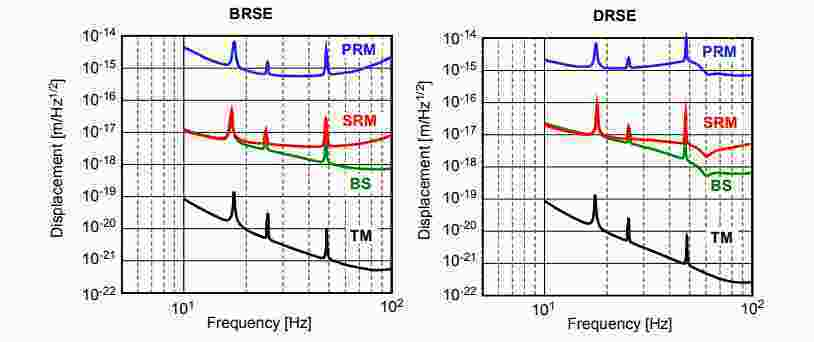
\includegraphics[width=0.7\linewidth]{figures/displacement_noise_requirement}
	\caption{Displacement noise requirements of the test mass (TM) (black), beamsplitter (BS) (green), signal recycling mirror (SRM) (red), and power recycling mirror (PRM) (blue), under boardband resonant sideband extraction configuration (BRSE) (Left) and detuned resonant sideband extraction scheme (DRSE) (Right). Retrieved from \cite{Sekiguchi:2016bmv}.}
	\label{fig:displacementnoiserequirement}
\end{figure}
As can be seen, the requirements of optics other than the TMs are much lower.
The displacement noise level of the BS and the SRM is at $10^{-17}~\mathrm{m}$, while that of the PRM is at $10^{-15}~\mathrm{m}$.
Table~.\ref{table:displacement_noise_requirement} summarizes the displacement noise of various optics at $10~\mathrm{Hz}$.
Therefore, the partial goal of suspension commissioning is to make sure these displacement noise levels requirement are met.
\begin{table}[!h]
	\centering
	\begin{tabular}{|c|c|}
		\hline
		& Displacement level ($\mathrm{m}/\sqrt{\mathrm{Hz}}$)\\
		\hline
		TM &  $1\times 10^{-19}$\\
		\hline
		BS &  $1\times 10^{-17}$\\
		\hline
		PRM & $2\times 10^{-15}$\\
		\hline
		PR2, PR3 & $1\times 10^{-15}$\\
		\hline
		SRM & $1\times 10^{-17}$\\
		\hline
		SR2, SR3 & $5\times 10^{-18}$\\
		\hline
	\end{tabular}
	\caption{Summary of longitudinal displacement noise level (at $10~\mathrm{Hz}$) of the optics including the folder mirrors of the recycling cavity (PR2, PR3, SR2, SR3). Retrieved from \cite{Sekiguchi:2016bmv}.}
	\label{table:displacement_noise_requirement}
\end{table}
The suspensions of the optics are designed specifically to attenuate the seismic noise at $10~\mathrm{Hz}$ to the displacement level specified in table.~\ref{table:displacement_noise_requirement} via passive isolation.
Therefore, the suspensions intrinsically satisfied these requirements already without any tweaking.
However, the main concern here is not about passive isolation.
Instead, it's about active isolation/feedback control, as we need to keep the control noise below these displacement level, while maintaining certain disturbance rejection capability.
This brings us to the other requirement: residual motion.

\subsection{Residual motion requirement \label{sec:residual_motion_requirement}}
In previous section, we discussed what are the requirements for KAGRA to be sensitive enough to become a gravitational wave detector.
Here, we will discuss the requirements for KAGRA to be an interferometric gravitational wave detector.
In particular, we will discuss velocity, angular fluctuation, and displacement level requirement.
Again, here we only briefly mention the rationale behind such requirements and readers are strongly recommended to read \cite{Sekiguchi:2016bmv} for detailed explanations.

\subsubsection{Residual velocity requirement}
In order for KAGRA to become an interferometric gravitational wave detector, the main optics must be manipulated to form various optical cavities, where feedback control is used to ``lock'' two mirrors at relatively stable separations.
The technique used is called Pound-Drever-Hall (PDH) technique \cite{doi:10.1119/1.1286663}.
To use this technique, the separation between two optics stay within the operating range where the control signal for using PDH technique becomes linear.
In \cite{Sekiguchi:2016bmv}, a velocity requirement of the is derived by considering the maximum actuation power of the TM coils.
Consider a case where the optics are moving towards the operating range.
As the optics enter the range, the actuators applies maximum force on the optics, causing the optics to decelerate maximally.
If the optics are put to halt before they exit the operating range, then lock-acquisition is achieved.
This only happens when the velocity of the optics is lower than a certain threshold, which we define as a requirement.
The velocity requirements the main optics are derived in \cite{Sekiguchi:2016bmv} and is summarized in table.~\ref{table:velocity_requirement}.
\begin{table}[!h]
	\centering
	\begin{tabular}{|c|c|}
		\hline
		& Velocity requirement (RMS) ($\mu\mathrm{m}/\mathrm{s}$)\\
		\hline
		TM, BS, SR &  $0.5$\\
		\hline
		PR &  $2$\\
		\hline
	\end{tabular}
	\caption{Summary of main optics' velocity requirement. Retrieved from \cite{Sekiguchi:2016bmv}.}
	\label{table:velocity_requirement}
\end{table}

\subsubsection{Residual angular displacement requirement}
Now, I don't really understand the rationale behind these angular fluctuation requirements\footnote{Please help me to write this section if you know the correction explanation. As far as I know, the angular fluctuation requirement comes from the fact that the interferometer needs to be aligned and that the beam spots are within good range around the center of the optics. But, I don't really know how people got those numbers.} and it seems that different sources suggests different things. I will simply report the requirements from some sources. 

In \cite{Sekiguchi:2016bmv}, it was reported that the RMS angles of the mirrors should not produce beam spot fluctuation on the optics by larger than an RMS value of $1~\mathrm{mm}$.
Using the beam paths as the lever arm, the angle fluctuation requirements are calculated and shown in table.~\ref{table:angular_fluctuation_requirement}.
\begin{table}[!h]
	\centering
	\begin{tabular}{|c|c|}
		\hline
		& Angular fluctuation RMS ($\mu\mathrm{rad}$)\\
		\hline
		TM &  $0.2$\cite{Sekiguchi:2016bmv, yuta_oplev}~/~$0.01$\cite{PhysRevD.88.043007, Mueller:05}\\
		\hline
		BS &  $4$\\
		\hline
		PRM & $45$\\
		\hline
		PR2 & $20$\\ 
		\hline
		PR3 & $2$\\
		\hline
		SRM & $25$\\
		\hline
		SR2 & $10$\\
		\hline
		SR3 & $1$\\
		\hline
	\end{tabular}
	\caption{Angular fluctuation requirements of the optics. Retrieved from \cite{Sekiguchi:2016bmv, yuta_oplev} unless otherwise specified.}
	\label{table:angular_fluctuation_requirement}
\end{table}
However, in another source regarding beam jittering at LIGO \cite{Mueller:05}, it's mentioned that the angular fluctuation requirement of the test masses at LIGO is $10^{-8}~\mathrm{rad}$.
The same value is also used to derive the wavefront sensor sensitivity requirement at KAGRA \cite{PhysRevD.88.043007}.
It's worth noting that both of these sources were also cited in \cite{Sekiguchi:2016bmv}.
So unless there's extra comment regarding this, let's just set the requirement for the TM to the lower one ($10^{-8}~\mathrm{rad}$) as a worst case scenario\footnote{There's a chance that we cannot confirm that we actually satisfied this requirement at the end of suspension commissioning as there's no sensors sensitive enough to measure such small level of fluctuation.Let's hope that our optical levers are sensitive enough}.

\subsubsection{Longitudinal displacement level requirement}
At last, the longitudinal displacement requirement was derived also from the maximum actuation power of the force coils at the TM stage.
Doing so, we assume that only these actuators are used during lock acquisition, but this may not be the case, so here again we are assuming a worst case scenario.
Table.~\ref{table:displacement_rms_requirement} summarizes the displacement RMS value requirement of the main optics in KAGRA.
\begin{table}[!h]
	\centering
	\begin{tabular}{|c|c|}
		\hline
		& Displacement RMS requirement ($\mu\mathrm{m}$)\\
		\hline
		TM &  $0.01$\\
		\hline
		BS &  $3.3$\\
		\hline
		SRM & $3.3$\\
		\hline
		SR2, SR3 & $1.6$\\
		\hline
		PRM & $560$\\
		\hline
		PR2, PR3 & $280$\\
		\hline
	\end{tabular}
	\caption{Longitudinal displacement RMS requirement of the optics. Retrieved from \cite{Sekiguchi:2016bmv}.}
	\label{table:displacement_rms_requirement}
\end{table}
This concludes the residual motion requirements for the core optics. 
So, the other half of the goal is to actively control the suspensions so requirements as shown in Table.~\ref{table:velocity_requirement}, \ref{table:angular_fluctuation_requirement}, and \ref{table:displacement_rms_requirement} are met, while not violating noise specification as shown in Table.~\ref{table:displacement_noise_requirement}.
In the following sections, we shall discuss/review some of the methods and techniques that can be used to achieve these goals.
We will also discuss some ways that we used to verify the satisfaction these requirements.

\subsection{Miscellaneous}
This section mainly refers to artificial requirements that are set in \cite{suspension_commissioning}.

\subsubsection{Seismic noise}
As a vibration isolation system, the main goal of the suspensions is to isolate the sole external disturbance, that is, the seismic disturbance.
Therefore, the optics must satisfy the displacement noise and residual motion requirements under the influence of a background seismic noise.
However, the residual motion of the optics vary with seismic noise level, which means that the performance of the suspension evaluated at a certain moment may not be the same at the other, as the seismic noise is dynamic.
So, we purpose an additional constraint here.
We require that the displacement noise and residual motion requirements to be satisfied under the influence of a disturbance equivalent to a background seismic noise at the $90^\mathrm{th}$ percentile level in the winter season.
The choice of this seismic noise meant to be conservative as it's considered a very violent disturbance.
To give some perspective of how the seismic noise level is, the seismic noise at the $90^\mathrm{th}$ percentile in KAGRA is shown in Fig.~\ref{fig:kagra_seismic_noise_90th_percentile} \cite{seismic_noise_kagra}.
\begin{figure}[!h]
	\centering
	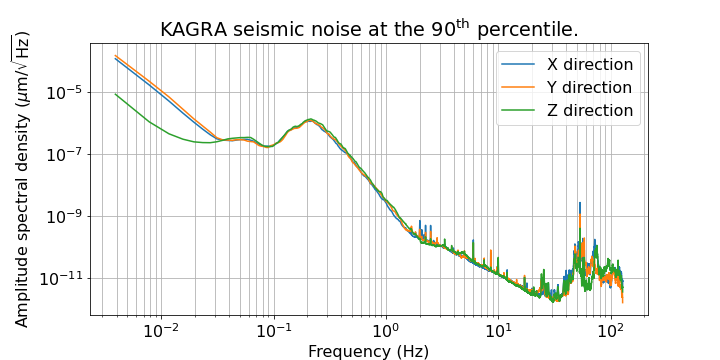
\includegraphics[width=0.7\linewidth]{figures/kagra_seismic_noise_90th_percentile.png}
	\caption{The amplitude spectral density of seismic noise in KAGRA at $90^\mathrm{th}$ percentile in $x$ (blue), $y$ (yellow), and $z$ (green) direction. Data retrieved from \cite{seismic_noise_kagra}.}
	\label{fig:kagra_seismic_noise_90th_percentile}
\end{figure}
As is mentioned, this is a conservative requirement, and it can be rare to observe such huge disturbance.
This means that it can be hard to test the suspension performance naturally.
To this end, as we shall see in later sections [ref later sections], we purpose to inject, using the actuators, artificial time series that has the same amplitude spectral density (ASD) of the measured seismic noise.

\subsubsection{Guardian}
Guardian is an automation system used in advanced LIGO (aLIGO) \cite{advanced_ligo_guardian}.
It's a platform where operators can program, using Python, certain operations that takes the suspensions from one defined states to another via certain defined paths.
The details of Guardian will not be discussed here, readers are strongly recommended to read the ``living'' document from aLIGO \cite{advanced_ligo_guardian}.
We will only briefly introduce what we're trying to achieve with Guardian and what people should expect.
Here, we will relay information given in \cite{suspension_commissioning, all_of_the_vibration}.
\begin{figure}[!h]
	\centering
	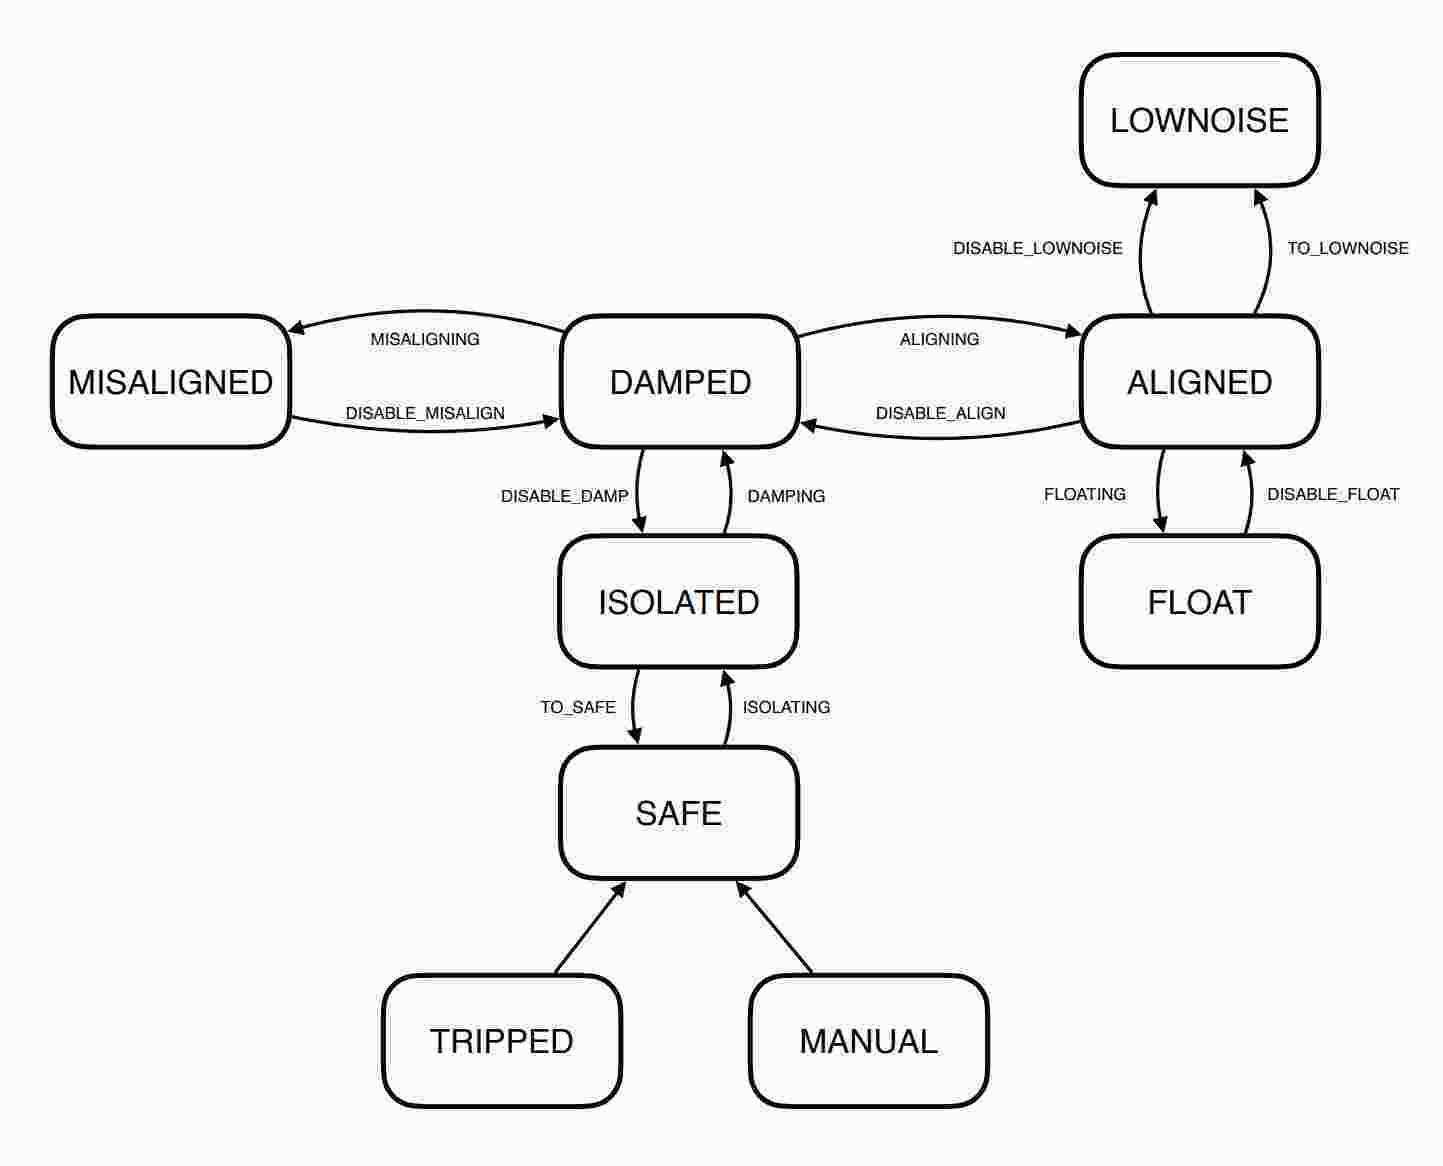
\includegraphics[width=0.7\linewidth]{figures/guardian}
	\caption{State-transition diagram of the (proposed?) VIS Guardian. Retrieved from \cite{all_of_the_vibration}}
	\label{fig:guardian}
\end{figure}
Fig.~\ref{fig:guardian} shows the (proposed?) state-transition diagram of the VIS Guardian.
As can be seen, there are 9 Guardian states, namely TRIPPED, MANUAL, SAFE, ISOLATED, DAMPED, MISALIGNED, ALIGNED, FLOATED, and LOWNOISE.
Here, description in \cite{all_of_the_vibration} is lacking so we will be further elaborating the behavior of these states.

In the TRIPPED state, as is indicated by the name of the state, the suspension is tripped.
This is triggered by a builtin watchdog system in the real-time model that monitors for abnormal behaviors.
The suspension can ``jump'' (In Guardian language) into this state from every other state.
This happens when the watchdog's tripped.

As for the MANUAL state, not sure what that means.
But my guess is that this is a state with the master switch turned on, so actuation signals can go through for measurement and diagnostic purposes.

In the SAFE state, actuation signals cannot go to the actuators, essentially immobilizing the suspension.

In the ISOLATED state, active isolation, usually at the stage closest to the ground (likely preisolator/inverted pendulum), is engaged.
The controls systems are engaged such that two things are achieved: 1) Coarsest alignment with integration action, and 2) Seismic noise suppression.
The controls at the higher stage will bring lower stages into operating point (e.g.centering the optical levers), but will perturb lower stage resonances via control noise injection.

In the DAMPED state, controls at the lower stages will be engage to suppress the these resonances.
At this point, the suspension should be able to satisfy the residual motion requirements as stated in Sec.~\ref{sec:residual_motion_requirement}.

In the ALIGNED state, the optics is steered to be coarsely aligned and is ready to be handed over to inferometer control.
Distinct from the ALIGN state, In the MISALIGN state, the optics is steered away from the aligned position.

At last, at the LOWNOISE state, controls that may compromise the detector sensitivity will be shut off or replaced by a lower noise version.
At this point, the suspension should satisfy the displacement noise requirements as stated in Sec.~\ref{sec:displacement_noise_requirement}.



	\section{Suspension Commissioning Tasks}
In this section, we will describe what are some specific tasks needed to be done in order to achieve the aforementioned goals in Sec.~\ref{sec:goal}.
In next section, Sec.~\ref{sec:suspension_commissioning_baseline_methods}, we will describe some of the mathematical details on how to complete these tasks, and how to evaluate the performance of the suspensions.
In the section after the next, Sec.~\ref{sec:suspension_commissioning_advanced_methods}, we will review some methods that has been proposed but are not considered baseline.
Here, we encourage readers to choose and implement the methods themselves.
There's no best method.
And, we should emphasize that it's not important to use the same methods for all suspensions, but rather, to evaluate all suspensions using the same evaluation methods.
As long as we have a consistent evaluation scheme that ensures the requirements are met, that's it needs for KAGRA to work.

\subsection{List of tasks}
We will provide a list of tasks here in this section.
Further elaboration will be provided in the next.
These tasks are defined with the assumption that we have healthy hardware and we have sensors (and actuators) calibrated, and they are listed in order.

\begin{enumerate}
	\item (If not done already) Sensor noise measurement (and modeling).  \label{item:sensor_noise_measurement}
	\item (If not done already) Seismic noise measurement (and modeling). Use a worst-case spectrum, e.g. $90^\mathrm{th}$ percentile seismic noise in the winter season. \label{item:seismic_noise_measurement}
	\item Control Matrices
	\begin{enumerate}
		\item Install initial sensing matrices and actuation matrices from first principles.
		\item Modify sensing matrices or apply ``diagonalization''/``decoupling'' matrices so the readout is mapped to the desired basis (Cartesian coordinate + Euler angles).
		\item (Optional) Modify actuation matrices or apply ``diagonalization''/``decouping'' matrices so the actuations are also in the desired basis.
	\end{enumerate}
	\item Inter-calibration of sensors.
	\item Further sensor noise reduction tasks, e.g. sensor fusion and sensor correction. Redo step \ref{item:sensor_noise_measurement}.
	\item Transfer function (TF) measurements and modeling. Do for
	\begin{itemize}
		\item Diagonal actuation TFs in a stage-by-stage basis, \label{item:diagonal_tf}
		\item (Optional) Cross actuation TFs in a stage-by-stage basis, and \label{item:cross_tf}
		\item TFs from each displacement to optics/test mass (TM) degrees of freedom. \label{item:displacement_to_optics_tf}
	\end{itemize}
	\item From the highest stage (closest to the ground) to lowest stage, design the control filter and do the following \label{item:design_control_filter}
	\begin{enumerate}
		\item Predict the closed-loop displacement level and
		\item estimate the residual motion and displacement noise contribution to the optics using
		\begin{itemize}
			\item the seismic noise measurement/open-loop displacement levels from step \ref{item:seismic_noise_measurement} or step \ref{item:open_loop_displacement_levels},
			\item sensor noise measurement from step \ref{item:sensor_noise_measurement}, and
			\item the displacement-to-optics displacements transfer functions from step \ref{item:displacement_to_optics_tf}.
		\end{itemize} 
		\item Check stability using stability critera (Nyquist plot and stability margins.) and transfer functions from step \ref{item:diagonal_tf}.
		\item If any of the above failed, tune the control filter.
		\item Install the control filters and close the loop.
		\item Measure open-loop displacement levels of the next stage (Keep the controls at upper stage engaged.) and move on the next stage. \label{item:open_loop_displacement_levels}
		\item Repeat step \ref{item:design_control_filter} until all local control-loops at all stages are closed.
	\end{enumerate}
	\item Measure the residual motion using the sensors at the optics stage as an out-of-loop sensor (Do not engage the control-loops that use the optics' sensors). If this fails, find the problematic stage and redo all controllers starting from there.
	\item (If there exists an interferometer) Measure actuation to DARM transfer function and measure the displacement noise. If this fails, find the problematic stage and redo all controllers starting from there.
\end{enumerate}

\subsection{Further elaboration}
In order to achieve the displacement noise and residual motion requirements, as stated in Sec.~\ref{sec:displacement_noise_requirement} and Sec.~\ref{sec:residual_motion_requirement} respectively, we need to rely on a so-called control system.
Here we assume readers have basic understanding on control systems and are comfortable at working with frequency/Laplace domain quantities.
If not, please refer to introductory textbooks such as \cite{modern_control_engineering} and \cite{control_engineering}.

A suspension has a lot of degrees of freedom (DoFs).
KAGRA's control topology requires each DoF to be independent from each other.
Therefore each DoF can be thought as a single-input-single-output (SISO) system as shown in Fig.~\ref{fig:generalcontrolblockdiagram}.
\begin{figure}[!h]
	\centering
	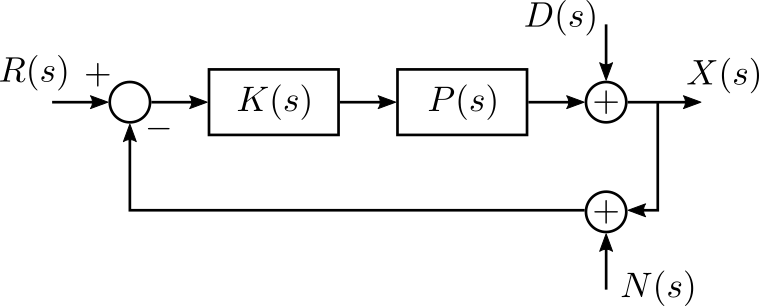
\includegraphics[width=75mm]{figures/general_control_block_diagram}
	\caption{Typical control block diagram of a single degree of freedom. $R(s)$: reference/setpoint, $D(s)$: external disturbance, $X(s)$: displacement, $N(s)$ sensing noise, $K(s)$: controller, $P(s)$: actuation transfer function.}
	\label{fig:generalcontrolblockdiagram}
\end{figure}
Now, we shall omit writing the bracket and assign capital letters to frequency/Laplace domain quantities and lower case letters for others.
Here, we define arbitrary functions $F(s)$ to be the Laplace transform of $f(t)$, where $s=\sigma+i\omega$ a complex number.
Typically, we analysis the functions by evaluating $s$ along the imaginary axis, i.e. frequency axis, so the functions we study here is closely related to the Fourier transform, and hence the amplitude spectral density, as we shall see later.
In Fig.~\ref{fig:generalcontrolblockdiagram}, $R$ is the setpoint, which is usually a static input at DC for coarse alignment purpose.
For most purposes in KAGRA's suspension, $R$ is considered to be $0$ at non-zero frequencies and therefore we will just mention it's existence but will not further discuss.
In the figure, $D$ is the external disturbance, that is, the open-loop spectrum of the displacement $X$\footnote{For a multiple stage suspension, $D$ is the displacement excited by motion at a higher stage.}.
$N$ is sensing noise, not sensor noise (we will properly define the meaning of $N$ later).
$K$ is the control filter, which is the filter that we need to design, and $P$ is the actuation transfer function of the suspension, which we need to model.

Here, the displacement reads
\begin{equation}
	X=\frac{1}{1+KP}\ D + \frac{KP}{1+KP}\ N.
	\label{eqn:X}
\end{equation}
From here, we shall define the proper definition of $N$ to be the limit of the displacement $X$ as the controller gain $K$ goes to infinity,
\begin{equation}
	N = \lim_{K\to\infty} X(K).
\end{equation}
So, it's not necessary sensor noise, but any residual signals present in the sensing readout\footnote{For example, the relative displacement sensors (LVDTs) at the preisolator of the Type-A and Type-B suspensions is coupled to ground motion, so the total sensing noise is a combination of the LVDT's intrinsic noise and seismic noise.}.
Continuing from Eqn.~\eqref{eqn:X}, the amplitude spectral density of $X$ is given by the quadrature sum of the filtered disturbance and sensing noise, i.e.
\begin{equation}
	X_\mathrm{ASD}(f) = \left[\left\lvert\frac{1}{1+KP}\right\rvert^2 D_\mathrm{ASD}^2(f) + \left\lvert\frac{KP}{1+KP}\right\rvert^2 N_\mathrm{ASD}^2(f)\right]^{\frac{1}{2}}.
\end{equation}
This is the quantity that we're interested in.
If this is the displacement of an upper stage, then we can estimate the displacement at the optics (TM) by
\begin{equation}
	X_\mathrm{ASD, TM}(f) = \left\lvert P_{X\to X_\mathrm{TM}}\right\rvert X_\mathrm{ASD}(f),
	\label{eqn:x_asd_tm}
\end{equation}
where $X_\mathrm{ASD, TM}(f)$ is the amplitude spectral density of the optics displacement $X_\mathrm{TM}$ and $P_{X\to X_\mathrm{TM}}$ is the transfer function from the displacement $X$ to the optics displacement $X_\mathrm{TM}$.

Once we can estimate the amplitude spectral density of the optics using Eqn.~\eqref{eqn:x_asd_tm}, we can tune 

\subsection{Control system preparatory tasks}
\subsubsection{Control matrices}
Now, before we can work with control systems, we need 
\subsection{Control tasks}


	\section{Suspension Commissioning Baseline Methods \label{sec:suspension_commissioning_baseline_methods}}
In this section, we will review some methods that can be used to tackle tasks as listed in Sec.~\ref{sec:list_of_tasks}.
This section will include ``baseline'' methods, which are some techniques that are considered to be the standard, or the fallback, methods that have been implemented previously or are simple enough that they must work.
They are sufficiently decent methods that should theoretically get the suspensions to satisfies the requirements.
These are also methods that has been used previously by various experts at KAGRA, so these shouldn't new to many of us.
However, these methods can be suboptimal.
For advanced methods, please refer to the next section, Sec.~\ref{sec:suspension_commissioning_advanced_methods}.

\subsection{Sensor noise measurement and estimation}
In this section we will describe the measurement and estimation of the intrinsic noise of displacement sensors and inertial sensors, and how to model them.

\subsubsection{Displacement sensors \label{displacement_sensors_baseline}}
Displacement sensors are usually relative displacement sensors that measure the differential displacement between the mounting point and an object.
Example sensors are Linear Variable Differential Transformer (LVDT) \cite{Akutsu:2021auw}, optical sensors and electromagnetic actuator (OSEM) \cite{Akutsu:2020efg, use_of_osems}, photo-reflective displacement sensors/photo sensors (PS), and optical levers (OpLev) \cite{sensing_matrices_oplev, length_sensing_oplev, optical_lever_for_kagra}.

In KAGRA's suspension, displacements sensors are non-contact sensors, i.e. the sensor doesn't affect the motion the sensing object, so the suspensions can swing freely to achieve passive seismic isolation.
However, this would mean that the sensing readout $Y$ contains the motion of the suspension, if the sensors are already installed, i.e.
\begin{equation}
	Y=X+N\,,
	\label{eqn:displacement_sensing_readout}
\end{equation}
where $X$ is the displacement readout and $N$ is the sensing noise.
Therefore, the only way to measure the sensor noise of the displacement sensors is to fix the suspension using the security structure, such that $X=0$.

Alternatively, we can measure the sensor noise before installation and apply proper calibration factors afterwards to convert the measurement units to displacement.
However, there might be error using this method, as there's no guarantee that the sensor noise retains the same before and after installation (or outside/inside vacuum/chamber).

Now, the aforementioned two methods can only be done before/during the installation stage.
If sensors are installed and in operation, there's no way to use these methods to measure the sensor noise of the displacement sensors\footnote{Can we use a three-channel correlation method?}.
But, approximation can still be done if have a model of the sensor noise.
This will be discuss in Sec.~\ref{sec:noise_modeling_baseline}.

\subsubsection{Inertial sensors}
In this section, we will describe techniques using correlation methods to measure sensor noise of inertial sensors \cite{technique_for_measurement_of_the_noise, Sleeman2006ThreeChannelCA}. Please also refer to appendix~\ref{appendix:spectral_density} for definitions and properties related to spectral densities.

Unlike displacement sensors, inertial sensors are self-contained sensors that are mounted to an object, whose motion are to be measured.
Some example sensors are geophone \cite{Sekiguchi:2016bmv}, accelerometers \cite{status_of_acc_development_2}, and seismometers \cite{trillium_compact_120-sv1}.
Calibrated inertial sensors output the velocity or the acceleration of the object which is relative to the object's inertial frame.
Because of this, sensor noise of inertial sensors cannot be measured by measuring the readouts when fixing suspension, as the readouts become the motion of the ground (effectively making the inertial sensor a seismometer.).
In any case, The readout of a single inertial sensor will be no different from that of Eqn.~\eqref{eqn:displacement_sensing_readout}.
Therefore, we cannot use single readout to estimate the sensor noise.

Instead, we rely on using multiple sensors and use correlation methods.
Now, let's assume that we have multiple sensors that reads $Y_i$, where $i=1,2,...K$, and $K$ is the total number of sensors.
If we place the sensors at the same location, they measure the same signal $X$.
Then, the sensor readouts becomes
\begin{equation}
	Y_i = XH_i + N_i\,,
	\label{eqn:inertial_sensing_readout}
\end{equation}
where $H_i$ is the transfer function from the signal to the sensing readout and $N_i$ is the sensor noise of the $i^\mathrm{th}$ sensor.

\paragraph{Two-channel method}

If we have sensors that have the same response and same power spectral density, then we can determine the sensor noises using only two sensors \cite{technique_for_measurement_of_the_noise}.
Let's say the sensors are well calibrated such that $H_i=1$, and assuming that the signal $X_i$ is uncorrelated with the noise $N_i$, then the power spectral density of the sensor readouts is simply
\begin{equation}
	P_{y_iy_i}(f) = P_{xx}(f) + P_{n_i n_i}(f)\,,
\end{equation}
and the cross power spectral density (CPSD) between $Y_i$ and $Y_j$ is
\begin{equation}
	\begin{split}
	P_{y_iy_j}(f) &= P_{xx}(f) + P_{xn_i}(f) + P_{n_ix}(f) + P_{n_in_j}(f) \\
	&= P_{xx}(f)\,,
	\end{split}
%	\label{eqn:p_yi_yj}
\end{equation}
where we assume $X$, $N_i$, and $N_j$ are uncorrelated for $i\neq j$ so their CPSDs are identically zero.
Following that, the coherence between sensor readout $Y_i$ and $Y_j$ is
\begin{equation}
	\begin{split}
	C_{y_iy_j}(f) &= \frac{\left\lvert P_{y_iy_j(f)}\right\rvert^2}{P_{y_iy_i}(f)P_{y_jy_j}(f)}\\
	&= \frac{P_{xx}(f)^2}{\left[P_{xx}(f)+P_{n_i n_i}(f)\right]\left[P_{xx}(f)+P_{n_j n_j}(f)\right]} \,.
	\end{split}
	\label{eqn:coherence_yi_yj}
\end{equation}
Here, if the power spectral densities of $N_i$ and $N_j$ is the same, i.e. $P_{n_in_i}(f)=P_{n_jn_j}(f)$, Eqn.~\eqref{eqn:coherence_yi_yj} further simplifies to
\begin{equation}
	C_{y_iy_j}(f) = \frac{P_{xx}(f)^2}{\left[P_{xx}(f)+P_{n_i n_i}(f)\right]^2}\,.
\end{equation}
Substituting $P_{y_i y_i}(f) = P_{xx}(f) + P_{n_i n_i}(f)$ and rearranging, we get
\begin{equation}
	\begin{split}
		C_{y_iy_j}(f)^\frac{1}{2} &= \frac{P_{xx}(f)}{P_{y_iy_i}(f)} \\
		P_{y_iy_i}(f)C_{y_iy_j}(f)^\frac{1}{2} &= P_{xx}(f) \\
		P_{y_iy_i}(f)\left[1-C_{y_iy_j}(f)^\frac{1}{2}\right] &= P_{y_iy_i}(f) - P_{xx}(f)\,.
	\end{split}
\end{equation}
Substituting $P_{n_i n_i}(f) = P_{y_i y_i}(f) - P_{xx}(f)$, finally we obtain
\begin{equation}
	\boxed{
		P_{n_i n_i}(f) = P_{y_iy_i}(f)\left[1-C_{y_iy_j}(f)^\frac{1}{2}\right]
	}\,\ .
	\label{eqn:p_ni_ni_2channel}
\end{equation}
And again, note that Eqn.~\eqref{eqn:p_ni_ni_2channel} only works if the two sensors are identical, i.e. having the same noise spectral density and are inter-calibrated such that the read a same coherent signal.

\paragraph{Three-channel method}

Now, if we don't have identical sensors, which is generally true, then we have to rely on a three-channel method that uses 3 sensors \cite{Sleeman2006ThreeChannelCA}.
The advantage of this method is that we can estimate the sensor noise of each individual sensor, even if they have completely different calibration, dynamics, and noise spectrum.
Recall the sensor readout Eqn.~\eqref{eqn:inertial_sensing_readout}, the cross power spectral density between the $i^\mathrm{th}$ and $j^\mathrm{th}$ sensors is
\begin{equation}
	P_{y_iy_j}(f) = P_{xx}(f)H_iH_j^*\,,
\end{equation}
where $H_j^*$ denotes the complex conjugate of the transfer function $H_j$ and $i\neq j$.
Again, we have assumed that the coherent signal $X$, the noises $N_i$ and $N_j$ are uncorrelated such that their CPSDs are zero.
If we have three sensors then we can have two cross power spectral density, $P_{y_iy_k}(f)$ and $P_{y_jy_k}(f)$, and $i,j,k=1,2,3$ and $i\neq j\neq k$.
Then, taking the ratio gives
\begin{equation}
	\frac{P_{y_iy_k}(f)}{P_{y_jy_k}(f)} = \frac{H_i}{H_j}\,.
	\label{eqn:p_yi_yj}
\end{equation}
The ratio between the PSD $P_{y_iy_i}(f)$ and CPSD $P_{y_jy_i}$ reads
\begin{equation}
	\begin{split}
	\frac{P_{y_iy_i}(f)}{P_{y_jy_i}(f)} &= \frac{P_{xx}(f)H_iH_i^*\ + P_{n_in_i}(f)}{P_{xx}(f)H_jH_i^*} \\
	&= \frac{H_i}{H_j} + \frac{P_{n_in_i}(f)}{P_{y_jy_i}(f)}\,.
	\end{split}
	\label{eqn:p_yi_yi_on_p_yj_yi}
\end{equation}
Now, substituting Eqn.~\eqref{eqn:p_yi_yj} into Eqn.~\eqref{eqn:p_yi_yi_on_p_yj_yi} and rearranging gives
\begin{equation}
	\boxed{
		P_{n_in_i}(f) = P_{y_iy_i}(f) - \frac{P_{y_iy_k}(f)}{P_{y_jy_k}(f)}P_{y_jy_i}(f)\,
	}\,\ ,
	\label{eqn:p_ni_ni_3channel}
\end{equation}
which expresses the PSD of the noise as the PSDs and the CPSDs of the measurements.

\textbf{Warning. The following paragraph is not from \cite{Sleeman2006ThreeChannelCA}, but is seemingly important.}

\paragraph{Modified three-channel method}

Let's inspect Eqn.~\eqref{eqn:p_ni_ni_3channel}.
Eqn.~\eqref{eqn:p_ni_ni_3channel} is an equation as written in \cite{Sleeman2006ThreeChannelCA} but is seemingly not directly implementable.
The second term in Eqn.~\eqref{eqn:p_ni_ni_3channel} are products of cross power spectral densities.
If we look at Eqn.~\eqref{eqn:p_yi_yj}, the CPSDs are expressed in products of transfer functions, are complex-valued series.
These features should note exist in a power spectral density as it's expected to be a real-valued frequency series.
To fix this problem, we propose to modify Eqn.~\ref{eqn:p_ni_ni_3channel} by taking the absolute value of the second term, i.e.,
\begin{equation}
	\begin{split}
	P_{n_in_i}(f) &\approx P_{y_iy_i}(f) - \left\lvert\frac{P_{y_iy_k}(f)}{P_{y_jy_k}(f)}P_{y_jy_i}(f)\right\rvert\\
	&= P_{y_iy_i}(f) - \frac{\left\lvert P_{y_iy_k}(f)\right\rvert}{\left\lvert P_{y_jy_k}(f)\right\rvert}\left\lvert P_{y_jy_i}(f)\right\rvert\,.
	\end{split}
	\label{eqn:modified_three_channel_noise}
\end{equation}
Recall that the definition of coherence function, first line of Eqn.~\eqref{eqn:coherence_yi_yj}, we can write express the absolute value of a cross power spectral density as
\begin{equation}
	\left\lvert P_{y_iy_j}(f)\right\rvert = C_{y_iy_j}(f)^{\frac{1}{2}}P_{y_iy_i}(f)P_{y_jy_j}(f)\,
	\label{eqn:absolute_cpsd}
\end{equation}
where $C_{y_iy_j}(f)$ is the coherence function between readouts $Y_i$ and $Y_j$.
Substituting Eqn.~\eqref{eqn:absolute_cpsd} into Eqn.~\eqref{eqn:modified_three_channel_noise} gives
\begin{equation}
	\boxed{
		P_{n_in_i}(f) \approx 	P_{y_iy_i}(f)\left[1-\left(\frac{C_{y_iy_k}(f)}{C_{y_jy_k}(f)}C_{y_jy_i}(f)\right)^\frac{1}{2}\right]
	}\,\ ,
	\label{eqn:modified_p_ni_ni_3channel}
\end{equation}
which is an expression very similar to Eqn.~\ref{eqn:p_ni_ni_2channel} and has convenient properties, i.e. coherence functions are symmetric $C_{ij}(f) = C_{ji}(f)$.

\paragraph{Examples and discussions}

We will demonstrate the use of these correlation methods in the form of a Jupyter notebook.
The notebook is available in the Kontrol library \cite{kontrol_noise_estimation}.
We will copy important results from the notebook.

In this setup, we have three sensors reading $y_1(t)$, $y_2(t)$, and $y_3(t)$ respectively.
These readouts follow the from of Eqn.~\eqref{eqn:inertial_sensing_readout}.
Furthermore, we assume the noises can be expressed as $N_i = G_iW_i$, where $G_i$ is the noise dynamics/transfer function and $W_i$ is unitary white noise, such that the noises are colored.
The sensors are assumed to be sensing a common signal $x(t)$ such the the sensors read
\begin{equation}
	Y_i = XH_i + G_iW_i,
\end{equation}
and $i=1,2,3$.
Now, let's assume that $H_1=H_2$ and $G_1=G_2$ so we use the two-channel method, i.e. Eqn.~\eqref{eqn:p_ni_ni_2channel} to get the PSD of $N_1$ and $N_2$.
As for $N_3$, we can use the modified three-channel method, i.e. Eqn.~\eqref{eqn:modified_p_ni_ni_3channel}.



\subsubsection{Noise modeling \label{sec:noise_modeling_baseline}}
\subsection{Control matrices}
\subsubsection{Sensing matrices}
\subsubsection{Actuation matrices}
\subsubsection{Frequency dependent matrices}
\subsection{Inter-calibration}
\subsection{Sensor fusion}
\subsection{Sensor correction}
\subsection{Transfer function measurement and modeling}
\subsection{Time series simulation of a given PSD}
\subsection{Controller design}


	\section{Suspension Commissioning ``Advanced'' Methods \label{sec:suspension_commissioning_advanced_methods}}
\subsection{Control optimization methods}
\subsection{PReQua and modal damping}
\subsection{Suspension characterization using dynamic mode decomposition}
\subsection{And More}
	\bibliographystyle{unsrt}
	\bibliography{main_bib}
	\begin{appendices}
	\section{Spectral density \label{appendix:spectral_density}}

\subsection{Cross power spectral density and power spectral density}
The cross power spectral density (CPSD) between a signal $x(t)$ and $y(t)$ is defined as
\begin{equation}
	P_{xy}(f) \equiv \int_{-\infty}^\infty\ R_{xy}(\tau) e^{-i2\pi f \tau}\ d\tau\,,
\end{equation}
where $f$ is the frequency, $i$ is the imaginary number, and
\begin{equation}
	R_{xy}(\tau) \equiv \lim_{T\to\infty}\frac{1}{T}\int_0^T\ x(t)y(t-\tau)\ dt
\end{equation}
is the correlation function between $x(t)$ and $y(t)$.
The power spectral density (PSD) of a single signal $x(t)$ is then defined as the cross power spectral density between the signal $x(t)$ and itself, i.e. $P_{xx}(f)$.

\subsection{Amplitude spectral density}
The amplitude spectral density of a signal x(t) is simply defined as
\begin{equation}
	\hat{x}(f) \equiv \left[P_{xx}(f)\right]^{\frac{1}{2}}\,.
\end{equation}

\subsection{Coherence}
The coherence between two signals $x(t)$ and $y(t)$ is then defined as
\begin{equation}
	C_{xy}(f) \equiv \frac{\left\lvert P_{xy}(f)\right\rvert^2}{P_{xx}(f)P_{yy}(f)}\,.
\end{equation}

\subsection{Sum of signals}
If we have two signals that can be expressed by superposition of other signals, i.e. $x(t)=x_1(t)+x_2(t)$ and $y(t)=y_1(t)+y_2(t)$, then the cross spectral density between $x(t)$ and $y(t)$ is
\begin{equation}
	\begin{split}
		P_{xy}(f) &= \lim_{T\to\infty}\frac{1}{T}\int_0^T\ \int_{-\infty}^\infty\  \left[x_1(t)+x_2(t)\right][y_1(t-\tau)+y_2(t-\tau)]\,e^{-i2\pi f\tau}\ dt \\
		&= P_{x_1y_1}(f) + P_{x_1y_2}(f) + P_{x_2y_1}(f) + P_{x_2y_2}(f)\,.
	\end{split} 
\end{equation}
\subsection{Uncorrelated signals}
If $x(t)$ and $y(t)$ are uncorrelated signals, then their correlation function $R_{xy}(\tau)$ and $R_{yx}(\tau)$ is 0, and so is their cross power spectral density.
For a signal that can be expressed a sum of two uncorrelation signals, $z(t)=x(t)+y(t)$, then its PSD is
\begin{equation}
	\begin{split}
		P_{zz}(f) &= P_{xx}(f) + P_{xy}(f) + P_{yx}(f) + P_{yy}(f)\\
		&= P_{xx}(f) + P_{yy}(f)\,.
	\end{split}
\end{equation}

\subsection{Transfer function}
The transfer function with input $x(t)$ and output $y(t)$ is can be estimated by
\begin{equation}
	P_{X\to Y} = \frac{P_{xy}(f)}{P_{xx}(f)}\,.
\end{equation}
\end{appendices}
\end{document}